\section{Introduction}
\label{sec:intro}

The main purpose of indoor scene layout estimation is to extract semantic boundaries among walls, ceiling and floor from a single image. It can be realized by obtaining corresponding semantic planes, as shown in Fig. \ref{fig:definition}. 


\begin{figure}[!ht]
	\centering
	\textsc{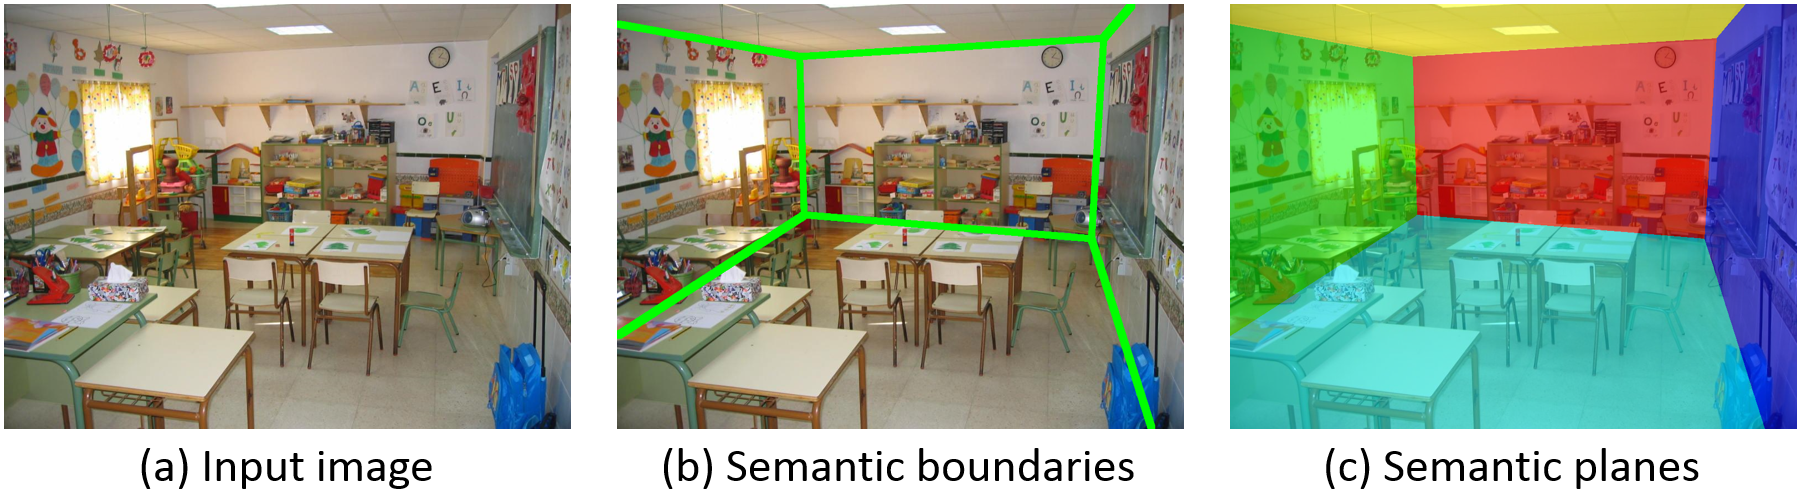
\includegraphics[width=8.5cm]{figure/def.png}}
	\caption{Illustration of the layout estimation problem. (a) Input image. (b) Layout estimation with semantic boundaries. (c) Layout estimation visulized with semantic planes.}
	\label{fig:definition}
\end{figure}


Room layout estimation is a fundamental problem for indoor scene understanding and plays a critical role in a diverse range of applications. For example, scene reconstruction, robot navigation and virtual reality. However, it is challenging that the distinctive clues such as room corners and layout boundaries are often occluded by objects. In addition to the occlusion problem, environmental factors like illumination variations, viewpoints shift, objects diversity and clutter can make the situation worse.


%%
In recent years, many researchers have made massive attempts to estimate indoor room layout from a single image. Conventional methods usually follow a proposing-ranking framework \cite{hedau2009recovering,wang2013discriminative,gupta2010estimating,hedau2010thinking}. Specifically, they first generate numbers of proposals by vanishing point detection and ray sampling. Then a ranking step using hand-crafted features is adopted to select the best hypothesis. Recent methods built on fully convulutional networks(FCNs) achieve impressive performance \cite{mallya2015learning,ren2016coarse,zhang2016learning,dasgupta2016delay,zhao2017physics}. Typically, the FCNs are trained to segment semantic surfaces or to predict boundaries among them. Followed by a postprocessing scheme, the output from FCNs are refined to be consistent with Fig.~\ref{fig:definition}(b)(c). End-to-End approach for room layout estimation also has been explored by \cite{LeeRoomNet17}. They employ an encoder-decoder network to delineate room layout structure using
2D keypoints. 

In this paper, we propose to enhance the FCN's ability for room layout estimation by fully utilizing the geometric information of the scene. Our pipeline is shown in Fig.~\ref{fig:pipeline}. First, we estimate depth and normal maps from a single image using network in \cite{eigen2015predicting}. Then we integrate these geometric hints to train a multi-channel FCN for semantic surface segmentation. At last, an extended post-processing algorithm based on \cite{dasgupta2016delay} is applied to generally refine the estimation results. We evaluate our method on two popular benchmark dataset. Experimental results demonstrate that our method is robust and effective for layout estimation even facing clutter and occlusion.






